\documentclass{article}
\usepackage{gvv-book}
\usepackage{gvv}
\usepackage{amsmath}
\usepackage{amsfonts}
\usepackage{tikz}
\usepackage{setspace}
\usepackage{gensymb}
\usepackage[cmex10]{amsmath}
\usepackage{amsthm}
\usepackage{mathrsfs}
\usepackage{txfonts}
\usepackage{stfloats}
\usepackage{bm}
\usepackage{cite}
\usepackage{cases}
\usepackage{subfig}
\usepackage{longtable}
\usepackage{multirow}
\usepackage{enumitem}
\usepackage{mathtools}
\usepackage{tikz}
\usepackage{circuitikz}
\usepackage{verbatim}
\usepackage[breaklinks=true]{hyperref}
\usepackage{tkz-euclide}
\usepackage{listings}
\usepackage{color}    
\usepackage{array}    
\usepackage{longtable}
\usepackage{calc}     
\usepackage{multirow} 
\usepackage{hhline}   
\usepackage{ifthen}   
\usepackage{lscape}     
\usepackage{chngcntr}
\usepackage{graphicx}
\usepackage{float}
\usepackage{multicol}
\usepackage[a4paper, left = 1.5cm, right = 1.5cm]{geometry}



\begin{document}

\begin{center}
\large
    \textbf{Samyak Gondane-AI25BTECH11029}
\end{center}
\date{}


\section*{Question}
Find the length of the median of the triangle with vertices \textbf{A}(0,0,6),\textbf{B}(0,4,0) and \textbf{C}(6,0,0).


\section*{Step 1: Midpoints of Opposite Sides}
\begin{align}
M_{BC} &= \frac{1}{2}(\vec{B} + \vec{C}) = \frac{1}{2} \myvec{4 + 6 \\ 0 + 0} = \myvec{5 \\ 0} \\
M_{AC} &= \frac{1}{2}(\vec{A} + \vec{C}) = \frac{1}{2} \myvec{0 + 6 \\ 6 + 0} = \myvec{3 \\ 3} \\
M_{AB} &= \frac{1}{2}(\vec{A} + \vec{B}) = \frac{1}{2} \myvec{0 + 4 \\ 6 + 0} = \myvec{2 \\ 3}
\end{align}

\section*{Step 2: Vectors Representing Medians}
\begin{align}
\vec{AM} &= M_{BC} - A = \myvec{5 \\ 0} - \myvec{0 \\ 6} = \myvec{5 \\ -6} \\
\vec{BM} &= M_{AC} - B = \myvec{3 \\ 3} - \myvec{4 \\ 0} = \myvec{-1 \\ 3} \\
\vec{CM} &= M_{AB} - C = \myvec{2 \\ 3} - \myvec{6 \\ 0} = \myvec{-4 \\ 3}
\end{align}

\section*{Step 3: Lengths of Medians}
Using the Euclidean norm:


\begin{align}
\|\vec{v}\| = \sqrt{x^2 + y^2}
\end{align}


\begin{align}
\|\vec{AM}\| &= \sqrt{5^2 + (-6)^2} = \sqrt{25 + 36} = \sqrt{61} \\
\|\vec{BM}\| &= \sqrt{(-1)^2 + 3^2} = \sqrt{1 + 9} = \sqrt{10} \\
\|\vec{CM}\| &= \sqrt{(-4)^2 + 3^2} = \sqrt{16 + 9} = \sqrt{25} = 5
\end{align}

\begin{figure}[H]
    \centering
    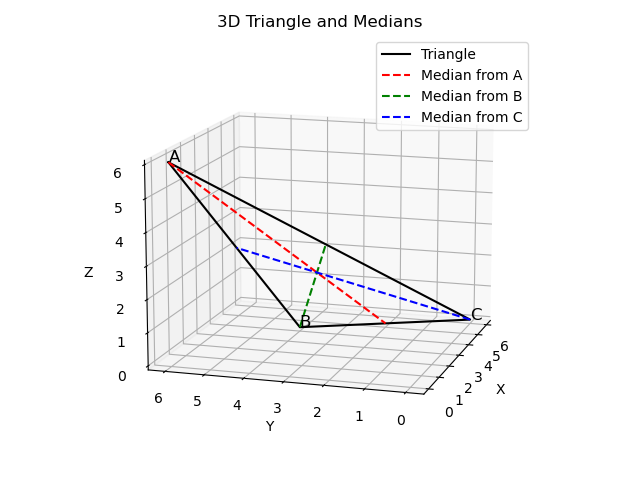
\includegraphics[width=0.75\linewidth]{figs/Figure_1.png}
    \caption{}
    \label{fig:fig1}
\end{figure}

\section*{Final Answer}


\begin{align}
\boxed{
\|\vec{AM}\| = \sqrt{61}, \quad
\|\vec{BM}\| = \sqrt{10}, \quad
\|\vec{CM}\| = 5
}
\end{align}



\end{document}
